%%%%%%%%%%%%%%%%%%%%%%%%%%%%%%%%%%%%%%%%%
% University/School Laboratory Report
% LaTeX Template
% Version 3.0 (4/2/13)
%
% This template has been downloaded from:
% http://www.LaTeXTemplates.com
%
% Original author:
% Linux and Unix Users Group at Virginia Tech Wiki
% (https://vtluug.org/wiki/Example_LaTeX_chem_lab_report)
%
% License:
% CC BY-NC-SA 3.0 (http://creativecommons.org/licenses/by-nc-sa/3.0/)
%
%%%%%%%%%%%%%%%%%%%%%%%%%%%%%%%%%%%%%%%%%

%----------------------------------------------------------------------------------------
%	PACKAGES AND DOCUMENT CONFIGURATIONS
%----------------------------------------------------------------------------------------

\documentclass{article}

\usepackage{mhchem} % Package for chemical equation typesetting
\usepackage{siunitx} % Provides the \SI{}{} command for typesetting SI units
\usepackage{hyperref}
\usepackage{graphicx} % Required for the inclusion of images
\usepackage{tabularx}
\usepackage{float}
\usepackage{algorithm}
\usepackage{algpseudocode}
\usepackage{bm}
\usepackage{multirow}% http://ctan.org/pkg/multirow
\usepackage{hhline}% http://ctan.org/pkg/hhline
\usepackage{caption}
\usepackage{subcaption}


\setlength\parindent{0pt} % Removes all indentation from paragraphs

\renewcommand{\labelenumi}{\alph{enumi}.} % Make numbering in the enumerate
% environment by letter rather than number (e.g. section 6)

%\usepackage{times} % Uncomment to use the Times New Roman font

%----------------------------------------------------------------------------------------
%	DOCUMENT INFORMATION
%----------------------------------------------------------------------------------------

\title{UC Davis STA 242 2015 Spring Assignment 4} % Title
\author{Wenhao \textsc{Wu}, 9987583} % Author name
\date{\today} % Date for the report

\begin{document}
\maketitle % Insert the title, author and date

% If you wish to include an abstract, uncomment the lines below

\section{Implementation of \texttt{crunBMLGrid()}}
In order to highlight the performance difference between R and C++
implementation of BML simulation, we implement the entire \texttt{crunBMLGrid()}
in C++. To do so, we made use of package `Rcpp'~\cite{}. The overall algorithm
design is very similar to the original R function \texttt{runBMLGrid()}.
However, at each step when we move all blue or red cars, the main operations are
executed in a for-loop instead of vectorized, as defined in our C++ function
\texttt{moveCars()}. As suggested by the example ``R vectorisation vs. C++
vectorisation'' in~\cite{}, one advantage of C++ for-loop implementation over
the R vecotrized operation is that it might need to create less intermediate
vector variables. In our design we embraced this idea by passing reference
variables to functions whenever possible and modifing them in-place (which may
not be possible in R), and the necessary intermediate variables
(\texttt{buffer\_loc\_next} and \texttt{buffer\_movable}) are also persistent.

\section{Verification}
We first verify qualitatively the behavior of BML model computed with our new
\texttt{crunBMLGrid()} routine. As in our previous assignment, We pick a
$r=100$, $c=99$ grid in which the number of blue cars and red cars are the same. After $N =
10000$ steps, the final states of the grid for $\rho = 0.2, 0.33, 0.38, 0.43,
0.5$ are plotted in Fig.~\ref{fig:final_state}, where we observe the same
chaotic phenomenon as the results computed with our original
\texttt{runBMLGrid()} routine.

We further verify that \texttt{crunBMLGrid()} and \texttt{runBMLGrid()}
returns identical result given the same input with package 'testthat'~\cite{}.
Besides the degenerated cases, in a $r=100$, $c=99$ grid we test 6 different cases
where there are different numbers of red and blue cars. For each case, we
randomly generate 5 instances of initial grid \texttt{g}. Our tests make sure
that the two routines returns identical result after $N =
10000$ steps for all 30 runs. We have also manually checked that, upon early
break from the outer for-loop due to grid lock when $\rho$ is large, the number of steps
executed before breaking are the same for both routines.

\begin{figure}[!t]
    \begin{minipage}[b]{0.5\linewidth}
      \centering
      \centerline{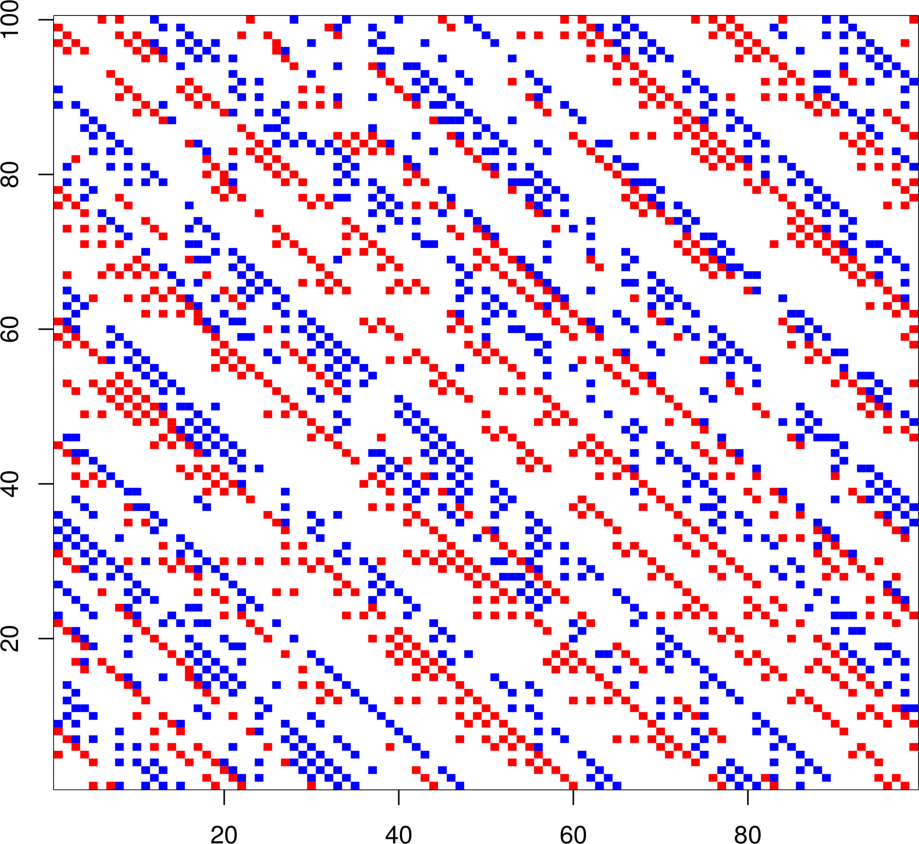
\includegraphics[width=6.0cm]{./figs/TestBehavior_100_99_10000_02_end.pdf}}
      \centerline{(a) $\rho = 0.2$}\medskip
    \end{minipage}
    \hfill
    \begin{minipage}[b]{0.5\linewidth}
      \centering
      \centerline{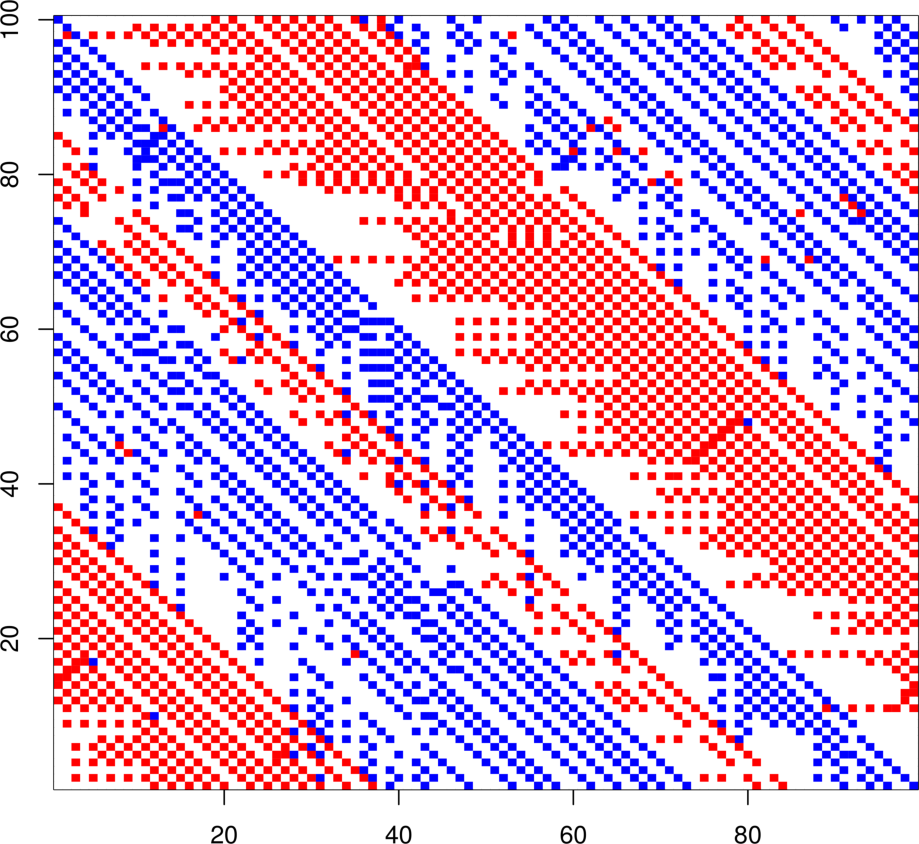
\includegraphics[width=6.0cm]{./figs/TestBehavior_100_99_10000_033_end}}
      \centerline{(b) $\rho = 0.33$}\medskip
    \end{minipage}
    \hfill
    \begin{minipage}[b]{0.5\linewidth}
      \centering
      \centerline{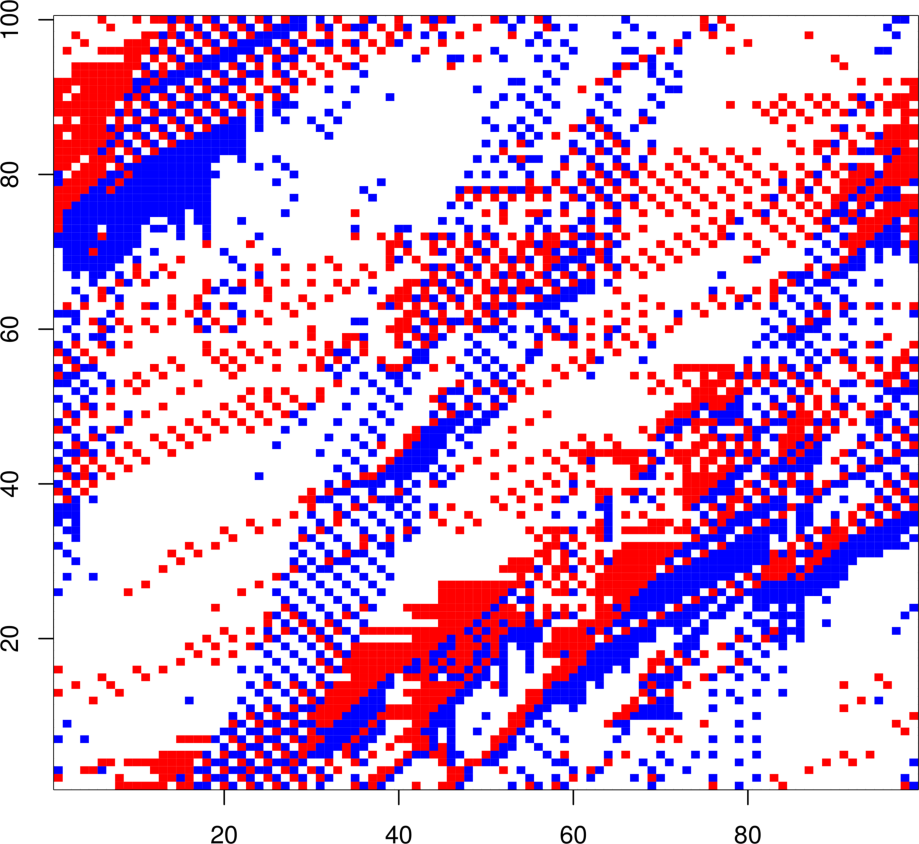
\includegraphics[width=6.0cm]{./figs/TestBehavior_100_99_10000_038_end}}
      \centerline{(c) $\rho = 0.38$}\medskip
    \end{minipage}
    \hfill
    \begin{minipage}[b]{0.5\linewidth}
      \centering
      \centerline{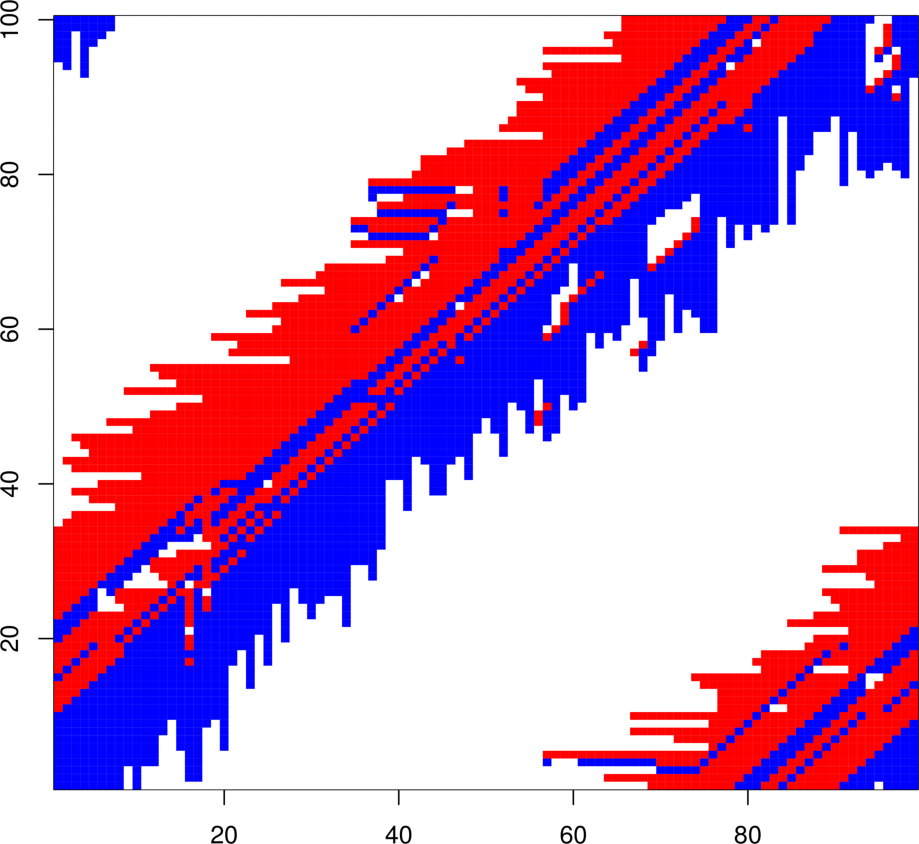
\includegraphics[width=6.0cm]{./figs/TestBehavior_100_99_10000_043_end}}
      \centerline{(d) $\rho = 0.43$}\medskip
    \end{minipage}
    \hfill
    \begin{minipage}[b]{1\linewidth}
      \centering
      \centerline{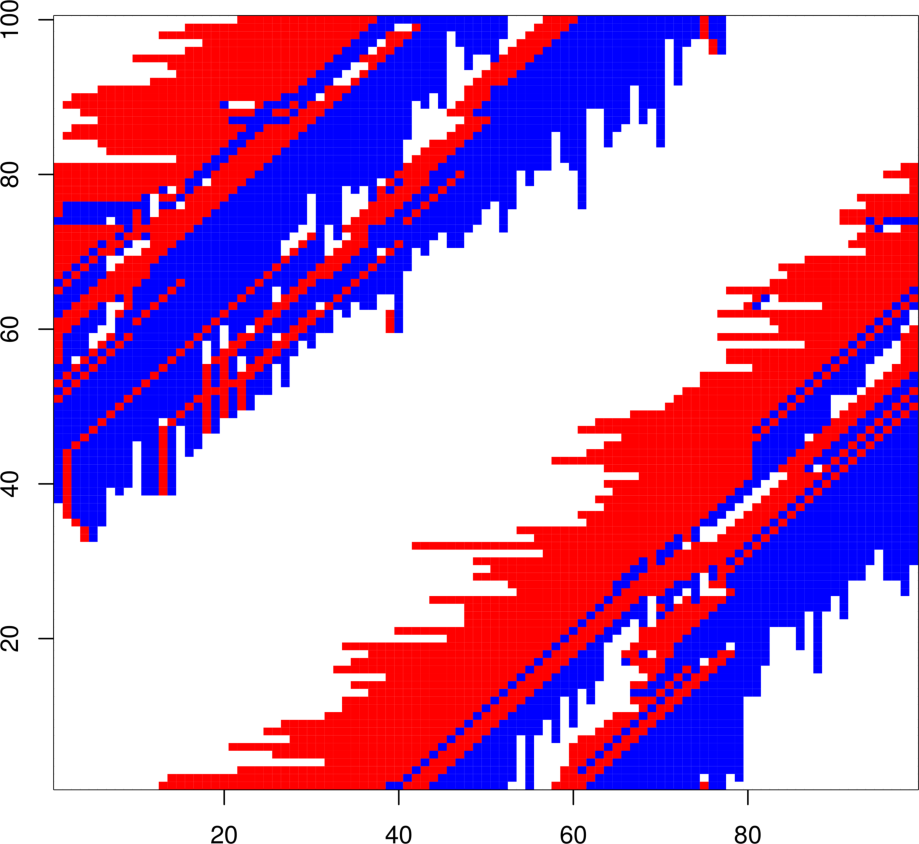
\includegraphics[width=6.0cm]{./figs/TestBehavior_100_99_10000_05_end}}
      \centerline{(e) $\rho = 0.5$}\medskip
    \end{minipage}
    \caption{Final state of a $100\times99$ grid with equal number of blue and
    red cars after 10000 steps for different car density $\rho$.}
    \label{fig:final_state}
\end{figure}


\section{Running Time Comparison with R's Vectorized Operation}
To compare the performance of \texttt{crunBMLGrid()} and \texttt{runBMLGrid()},
we measure the running time of both functions for $r=c=128,256,512,1024$ and
$\rho=0.1,0.2,9.3,0.4,0.5,0.6,0.7$. For each of the $4\times7=28$ settings we
randomly generate 10 initial grids and apply both \texttt{crunBMLGrid()} and
\texttt{runBMLGrid()} on them and record the average running time. We also fix
the number of steps to $N=10000$ and have the same number of red and blue cars
in the grid. Again we run this test on a Dell Precision T1700 workstation
equipped with 16GB DDR3 RAM and a Core i7-4790K CPU in Ubuntu 14.04 OS. The
average running time in seconds and the relative speed up from
\texttt{runBMLGrid()} to \texttt{crunBMLGrid()} are plotted in Fig.~\ref{fig:running_time}
and Fig.~\ref{fig:speed_up}, repectively. The original data of
Fig.~\ref{fig:running_time} is also provided in the Appendix. In our test cases,
the speed up is from 3x to 10x. In general, the larger the edge length, the
smaller the speed up is. Surprisingly, the speed up for cases where there is no
grid lock detected is significantly higher than the cases where there is grid lock
and early breaks. Our guess is that the initialization part of the routine takes
a larger portion of time in \texttt{crunBMLGrid()} than in
\texttt{runBMLGrid()}.

\section{Conclusion}
Based on the above results, our conclusion is
\begin{itemize}
    \item There is a speed up from rewritting R's vectorization-based
    routines into C++ for-loop based routines in this assignment.
    \item However, in my opinion a C++ implementation is not worthwhile. In our
    case, the performance gain is not so significant, thus unless we are doing
    really time-consuming simulations, using R's vectorization-based
    routines is more advantageous in terms of agile development. Also, in order
    to maximize the speed up, we have rewritten the entire \texttt{runBMLGrid()}
    with C++. As a result, we cannot make the same function to return different
    types of values for different inputs and it is more difficult to add other
    functionalities (such as animation) to the function.
\end{itemize}

\begin{figure}[t]
    \centering
    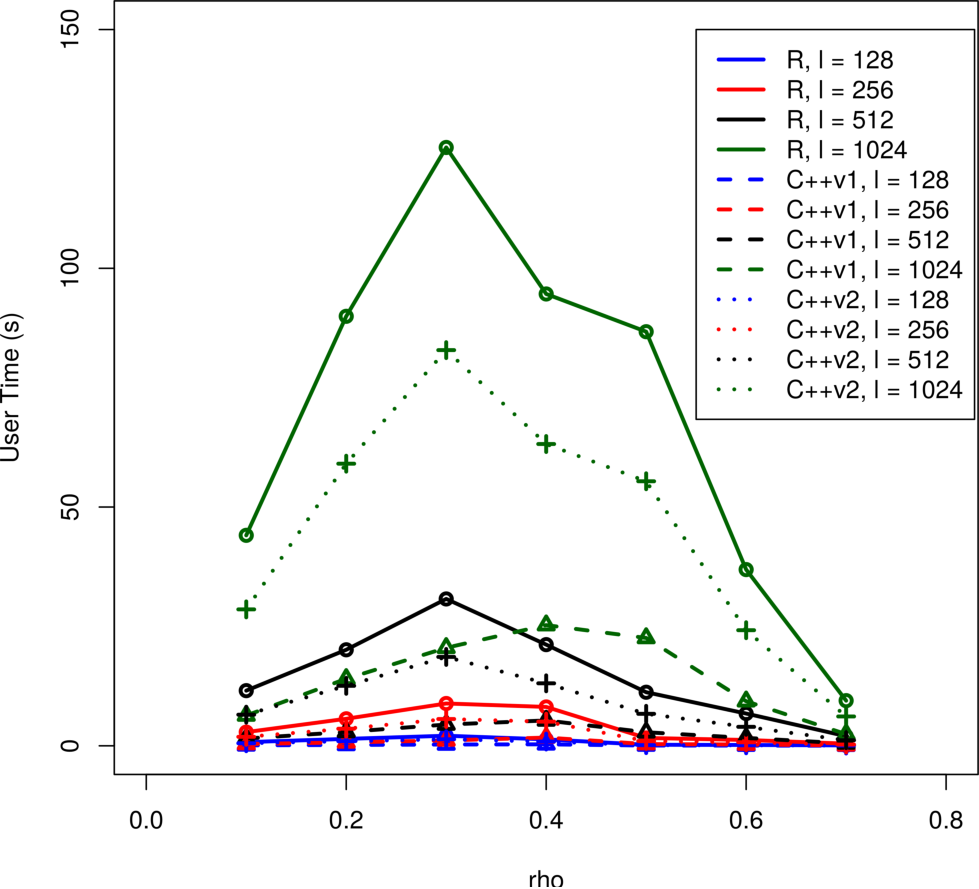
\includegraphics[width=3.5in]{figs/TestRunningTime.pdf}
    \caption{User time of \texttt{crunBMLGrid(g, 10000)} \texttt{runBMLGrid(g,
    10000)} averaged over 10 repetitions for $\rho=0.1,0.2,9.3,0.4,0.5,0.6,0.7$
    and $r=c=128,256,512,1024$.}
    \label{fig:running_time}
\end{figure}

\begin{figure}[t]
    \centering
    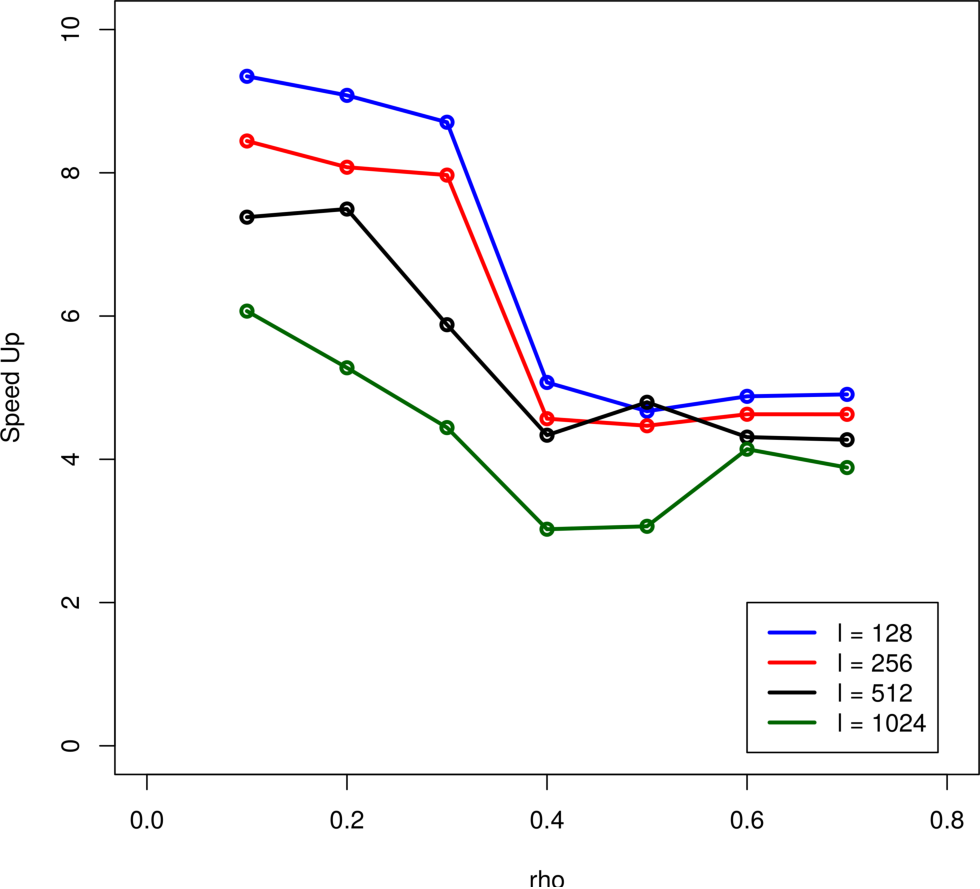
\includegraphics[width=3.5in]{figs/SpeedUp.pdf}
    \caption{Relative speed up by rewriting the R routine with C++.}
    \label{fig:speed_up}
\end{figure}

\section{Appendix A: Running Time Results}

\section{Appendix B:}
%\pagebreak
%	BIBLIOGRAPHY
%----------------------------------------------------------------------------------------

\bibliographystyle{unsrt}
\bibliography{myrefs}

%----------------------------------------------------------------------------------------


\end{document}